\documentclass[12pt]{article}
\usepackage{amssymb,mathrsfs, amsmath,amsfonts}
\usepackage{mathtools}
\usepackage{graphicx}
\usepackage{enumitem}
\usepackage{braket}
\usepackage{hyperref}
\graphicspath{ {./ps1-assets/}{./exercises/handwritten/ps1/ps1-assets/} }

\title{Problem Set 1}
\author{CSE 468}
\date{\today}

\begin{document}

\maketitle

\noindent \textbf{Note:} Many of these problems use \href{https://lab.quantumflytrap.com/lab}{this link}.

\begin{enumerate}[font=\bfseries]
    \item (35 points) Create the following setup in your own workspace.\\
    \[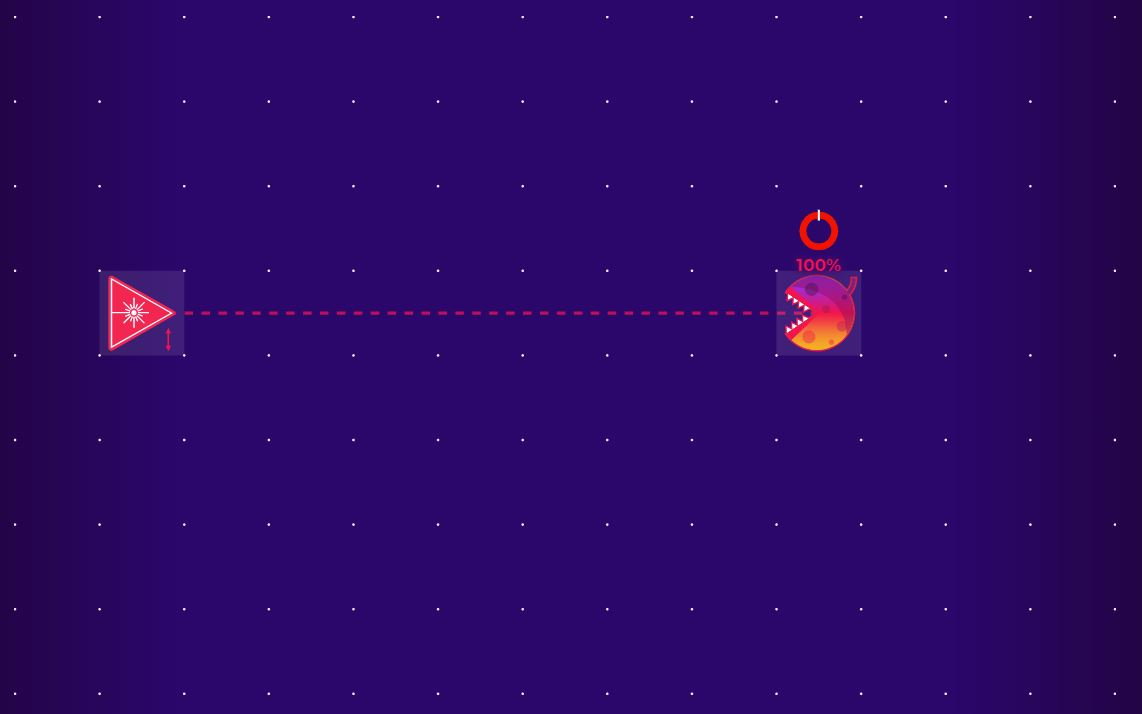
\includegraphics[scale=0.4]{easyFilter}\]
    \begin{enumerate}
        \item Using only polarizing filters create a configuration such that the detector only detects 6.25$\%$ of the initial photons. Please describe your configuration.
        \item Describe a general strategy using only polarizing filters that causes the detector to detect only $n\%$ of the initial photons. You may assume $n \leq 100$ and $n = \frac{100}{2^k}$ with $k\in\mathbb{Z}^+$.
        \item There is only one path in this configuration so we can use state to represent the polarization of the photons. Let $\ket{0} = \begin{pmatrix}1 \\ 0 \end{pmatrix}$ represent photons completely oriented in the horizontal direction. Similarly, let $\ket{1} = \begin{pmatrix}0 \\ 1 \end{pmatrix}$ represent photons completely oriented in the vertical direction. Note we can characterize any state of these bases by a single parameter $\theta$ as follows: $\ket{\psi} = \cos{\theta}\ket{0} + \sin{\theta}\ket{1}$. Assume the photon source outputs photons completely oriented in the vertical direction. Using this notation give the matrix that represents a polarizing filter oriented in the vertical direction.
        \item Given some state $\ket{\psi}$, what is the probability, in terms of $\theta$, that the photon will pass through a vertically oriented filter?
        \item Give the matrix that describes a general polarizing filter oriented $\theta$ degrees from the origin.
        \item Using the above notation, describe the state of your system before any filters are applied, after the first filter is applied, and after the second filter is applied.
        \item Does applying a vertical filter, then a horizontal filter, and then a filter oriented 45 degrees from the origin produce the same result as applying a vertical filter, then a filter oriented 45 degrees from the origin, and then a horizontal filter? Why or why not?
    \end{enumerate}
    \item (6 points) Create the following setup in your own workspace.
    \[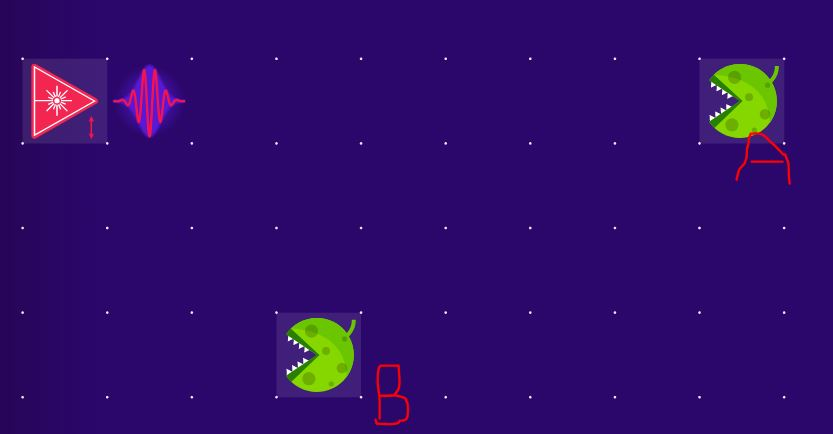
\includegraphics[scale=0.6]{beamSplit}\]
    Read about the polarizing beam splitter \href{https://lab.quantumflytrap.com/info/polarizing-beam-splitter}{here} and understand how it behaves with various inputs.
    \begin{enumerate}
        \item Using only polarizing beam splitters and polarizing filters, create a configuration such that the probability of measuring a photon at Receiver A and the probability of measuring a photon at Receiver B are both greater than zero.
        \item What is the maximum possible combined probability of a photon arriving at Receiver A or Receiver B? Why?
    \end{enumerate}
    \item (6 points) Recreate the initial configuration of Question 2. Read about the sugar solution tool \href{https://lab.quantumflytrap.com/info/sugar-solution}{here}.
    \begin{enumerate}
        \item Using only sugar solutions and polarizing beam splitters create a configuration such that the probability of measuring a photon at Receiver A and the probability of measuring a photon at Receiver B are both greater than zero.
        \item What is the maximum possible combined probability of a photon arriving at Receiver A or Receiver B? Why?
    \end{enumerate}
    \item (4 points) Go to the experimental setups section (in the top right menu). Choose the Quantum coin flip experiment. Click the detections mode in the bottom left and then click Play x100 and click run. This will run the experiment 100 times, keeping track of the number of photons that arrive at each receiver. 
    \begin{enumerate}
        \item How many counts should we expect to see in each receiver? 
        \item Run the experiment and report your results. Do your results match your predictions? Why or why not?
    \end{enumerate}
    \item (5 points) Consider the setup below.
    \[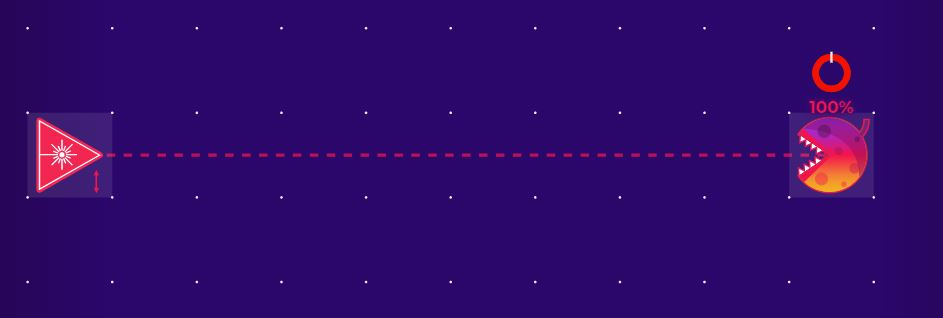
\includegraphics[scale=0.6]{rotate10}\]
    This website only allows us to rotate polarizing filters in increments of 45 degrees. Let's imagine that we were able to rotate polarizing filters in increments of 10 degrees.
    \begin{enumerate}
        \item How many polarizing filters could we place between the photon source and receiver and still expect to see at least 50\% of the initial photons in the receiver? Note we also require that consecutive filters have different rotations (i.e. you cannot just place infinite filters with the same rotation).
    \end{enumerate}
    \item (Bonus, up to 3 points) Write one interesting question related to the content of this homework, and indicate the correct answer. The question can be multiple-choice or free-response.  Interesting questions get credit here;  sufficiently good questions might appear on an exam.
\end{enumerate}



\end{document}
